\documentclass[11pt]{beamer}
\let\Tiny=\tiny
\usepackage[utf8]{inputenc}
\usepackage[T1]{fontenc}
\usepackage[final]{pdfpages} %permet d'insérer des pages pdf
\usepackage[french]{babel}
\usepackage{lmodern}

\usetheme{Frankfurt}
\useoutertheme[subsection=false]{smoothbars}
\useinnertheme[shadow=true]{rounded}
\usecolortheme{orchid}
\usecolortheme{whale}

% Ce package permet d'afficher correctement des URL dans un document LaTeX.
% Un URL contient toujours le caract<E8>re : (deux points). Or ce caract<E8>re
% devient actif en fran<E7>ais. Il faut donc momentan<E9>ment d<E9>sactiver ce
% caract<E8>re lors de l'utilisation de la commande \url
\usepackage{url}
\urlstyle{sf}

% Pour les smileys
\usepackage{wasysym}

% Pour les panneaux de signalisation
\usepackage{fourier-orns}

% Pour justifier le texte dans une frame
\usepackage{ragged2e}

% Pour pouvoir "cacher" des slides
\usepackage{ifthen}
\newboolean{includeannex}
\setboolean{includeannex}{false}
\newcommand{\ifannex}[1]{\ifthenelse{\boolean{includeannex}}{#1}{}} 

\usepackage{amsmath}
\usepackage{amsfonts}
\usepackage{amssymb}


% ---------------------------------------------------
%   Données pour le titre
% ---------------------------------------------------

\title{De-anonymisation de données et vie privée : étude d'un modèle de graphes aléatoires.}
\author{
  Clément Lalanne, \texttt{clement.lalanne@ens.fr, \\ D\'epartement d'informatique de l'ENS,\\ \'Ecole normale sup\'erieure,\\ PSL Research University,\\ 75005 Paris, France}
\\ Encadré par 
\\ Florian Simatos, \texttt{florian.simatos@isae-supaero.fr, \\ D\'epartement d'Ing\'enierie des Systèmes Complexes, \\ ISAE-SUPAERO, \\ 31400 Toulouse, France}
}
\date{}

\newcommand{\confname}{TIPE}

% ---------------------------------------------------

\definecolor{coultitre}{rgb}{0.33,0.44,0.55}  % bleu pétrole (#546F8B)
\setbeamercolor{structure}{fg=coultitre}

\definecolor{coulimportant}{rgb}{0.85,0.07,0.07} % rouge/brun (#B33333)
\setbeamercolor{alerted text}{fg=coulimportant}

% ---------------------------------------------------
% ---------------------------------------------------

\colorlet{mygrey}{black!50!white}

\setbeamertemplate{footline}{
  \leavevmode
  \hbox{
    \hspace*{-0.2cm}
    \begin{beamercolorbox}[wd=.15\paperwidth,ht=2.25ex,dp=1ex,center]{section in head/foot}%
      \usebeamerfont{sidebar}\color{white}\insertshortauthor\hskip2ex
    \end{beamercolorbox}%
    \begin{beamercolorbox}[wd=.75\paperwidth,ht=2.25ex,dp=1ex,center]{section in head/foot}%
      \usebeamerfont{sidebar}\color{white}\insertshorttitle
    \end{beamercolorbox}%
    \begin{beamercolorbox}[wd=.11\paperwidth,ht=2.25ex,dp=1ex,center]{section in head/foot}%
      \usebeamerfont{sidebar}\color{white}\insertframenumber{} / \inserttotalframenumber\hspace*{2ex}
    \end{beamercolorbox}%
  }
  \vskip0pt
}

\setbeamertemplate{navigation symbols}{}
% ---------------------------------------------------
% ---------------------------------------------------
% Début du document
% ---------------------------------------------------
% ---------------------------------------------------

\begin{document}

\def\vdep{\succ}
\def\dep{\rightarrow}
\def\deparrow#1{\lower 2 pt \hbox{$~\stackrel{#1}{\longrightarrow}~$}}
\def\anydep{\leadsto}
\def\ivdep{\vdep^*}
\def\idep{\rightarrow^*}
\def\ideparrow#1{\lower 2 pt \hbox{$~\stackrel{#1}{\longrightarrow}${${}^*$~}}}
\def\ianydep{\leadsto^*}


\newtheorem*{theoreme}{Théorème}
\newtheorem*{defi}{Définition}
\newtheorem*{proposition}{Proposition}
\newtheorem*{preuve}{Preuve}
\newtheorem*{lemme}{Lemme}
\newtheorem*{remarque}{Remarque}
\def\card{\mathop{\rm card}}

%--------------------------------------------------------------------
%--------------------------------------------------------------------
% Page de garde
%--------------------------------------------------------------------
%--------------------------------------------------------------------

\begin{frame}
\titlepage
\vspace{-2cm}
\end{frame}

\section*{Introduction.}

\begin{frame}
\frametitle{\insertsection}
Anonymiser un réseau social avant d'en publier les informations n'est parfois pas suffisant pour garantir la vie privée de ses utilisateurs. Par exemple en 2006 une partie des personnes ayant participé à un sondage de Netflix ont pu être retrouvées. Cependant ces informations structurelles peuvent être utilies à différents organismes ainsi il faut trouver la limite entre clarté et opacité des informations révélées.
\end{frame}

\begin{frame}
	\frametitle{\insertsection}
	\tableofcontents[hideothersubsections]
\end{frame}

\section{Présentation du problème}

\subsection{Problème de de-anonymisation}

\begin{frame}
\frametitle{\insertsubsection}


\begin{figure}[!h]
	\centering
	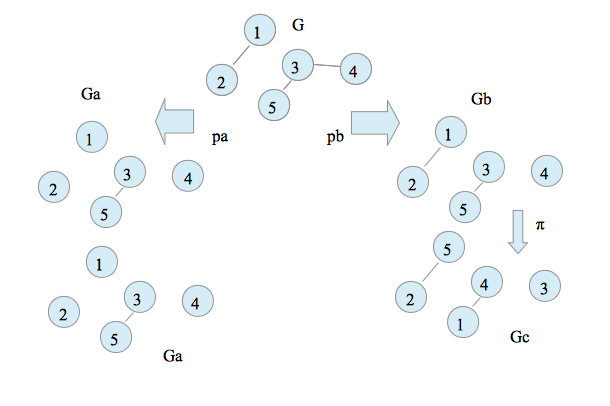
\includegraphics[scale=0.5]{01.png} \\
	\end{figure}	

\end{frame}

\subsection{Un premier modèle de graphes}

\begin{frame}
\frametitle{\insertsubsection}

Le premier modèle de graphes sur lequel nous allons étudier le problème de de-anonymisation est le modèle d'Erdös-Rényi. Dans le modèle $G(n,p)$ un graphe est construit sur un ensemble de $n$ sommets et chaque arête y apparaît indépendement avec probabilité $p$. De plus dans toute la suite nous ne considèrerons que le cas symétrique $p_a = p_b = s$

\end{frame}

\section{Mise en perspective des différents résultats}

\subsection{Résultats fondementaux}

\begin{frame}
\frametitle{\insertsubsection}
Une première idée est de prendre un identificateur qui minimise globalement le nombre d'erreurs. Dans leurs travaux, Pedarsenni et Grossglauser utilisent l'identificateur suivant :
\[
PG((g_c,g_b)) = argmin_{\pi} \Delta(g_c \circ A(\pi^{-1}), g_b)
\]
\[
\Delta(g_1,g_2) = \sum_{e \in \binom{[n]}{2}} |g_1(e)-g_2(e)|
\]

\end{frame}

\begin{frame}
\frametitle{\insertsubsection}
Ils trouvent alors le résultat fondamental suivant :

\begin{theoreme}
Pour le problème de de-anonymisation avec $s = \omega(1)$ et $p \rightarrow 0$, si $ps \frac{s^2}{2-s} \geq 8\frac{\log n + \omega(1)}{n}$ alors asymptotiquement presque sûrement (a.p.s.) $PG$ réussit à retrouver $\pi$.
\end{theoreme}

Plus récement, Cullina et Kiyavash améliorent ce résultat en trouvant une borne d'impossibilité de de-anonymiser.

\begin{theoreme}
Pour le problème de de-anonymisation avec $s = \omega(1)$ et $p \rightarrow 0$, si $ps^2 \geq 2\frac{\log n + \omega(1)}{n}$ alors asymptotiquement presque sûrement (a.p.s.) $PG$ réussit à retrouver l'identité.
Si $(G_a,G_b) \sim ER(n,p,s)$ avec $p \rightarrow 0$ et $ps^2 \leq \frac{\log n - \omega(1)}{n}$ alors tout de-anonymiseur réussit avec probabilité $o(1)$
\end{theoreme}

\end{frame}

\subsection{Idée de preuve et estimateur MAP}

\begin{frame}
\frametitle{\insertsubsection}
\[
P(I \text{ réussit}) = \]\[\sum_{(g_c,g_b)} P((G_c,G_b) = (g_c,g_b)) P(\Pi = I((g_c,g_b)) |(G_c,G_b) = (g_c,g_b))
\]
\[
MAP((g_c,g_b))= argmax_{\pi} P(\Pi = \pi |(G_c,G_b) = (g_c,g_b))
\]
\end{frame}

\begin{frame}
\frametitle{\insertsubsection}
\begin{lemme}
Si $(G_a,G_b) \sim ER(n,p,s)$ alors :
\[
P(\Pi = \pi|(G_c,G_b) = (g_c,g_b)) \propto (\frac{p_{10}p_{01}}{p_{11}p_{00}})^{\frac{1}{2} \Delta(g_c \circ A(\pi^{-1}), g_b)}
\]
avec
\[
p_{11} = ps^2 
\]
\[
p_{10} = p_{01} = ps(1-s)
\]
\[
p_{00} = 1 - p(2s-s^2)
\]
\end{lemme}
\end{frame}



\subsection{De-Anonymisation avec graine}

\begin{frame}
\frametitle{\insertsubsection}
\begin{theoreme}
Si $(G_a,G_b) \sim ER(n,p,s)$ avec $ps^{2}$ $\leq$ $\frac{\log n - c_n}{n}$ et $c_n$ $\rightarrow$ $\infty$ alors tout identificateur utilisant une seed de taille au plus $\frac{1}{2} \exp(\frac{c_n - ps^{2} \log n}{1-ps^{2}}) - 1$ réussit avec probabilité au plus $\frac{1}{2}$. Si de plus la taille de la seed est en $o( \exp(\frac{c_n - ps^{2} \log n}{1-ps^{2}}))$ Alors l'identificateur réussit avec une probabilité $o(1)$.
\end{theoreme}
\begin{theoreme}
Si $(G_a,G_b) \sim ER(n,p,s)$ avec $ps^{2}$ $\leq$ $\frac{\log[(1-l) n] - c_n}{n}$ et $c_n$ $\rightarrow$ $\infty$ alors tout identificateur utilisant une seed pour laquelle chaque sommet y apparaît avec probabilité $l$ indépendement des autres réussit avec probabilité $o(1)$. 
\end{theoreme}
\end{frame}

\subsection{$(1-\epsilon)$-De-Anonimisation}

\begin{frame}
\frametitle{\insertsubsection}
\begin{theoreme}
Soit $\epsilon \in ]0,\frac{1}{2}[$. Si $(G_a,G_b)$ $\sim$ $AER(n,p,s)$ avec $ps^2 \leq \frac{\log(\frac{1}{2 (\delta + \epsilon)})}{n}$ pour $\delta \in ]\epsilon, \frac{1}{2}[$ alors tout $(1-\epsilon)$-de-anonymiseur réussit avec probabilité $o(1)$.
\end{theoreme}
\end{frame}

\section{De-Anonymisation pratique}

\begin{frame}
\frametitle{Algorithme gloute de Korula et Lattanzi}
\begin{defi}
Une paire de sommets $(u_a,u_b)$ est avec $u_a \in G_a$ et $u_b \in G_b$ est dit témoin de similarité de la paire $(v_a,v_b)$ avec $v_a \in G_a$ et $v_b \in G_b$ si $u_a \in N_a(v_a)$, $u_b \in N_b(v_b)$ et $u_a$ a été associé à $u_b$.
\end{defi}
\end{frame}

\begin{frame}[fragile]
\frametitle{\insertsubsection}

\begin{scriptsize}
\begin{verbatim}
Entrée : Deux graphes G_a et G_b, Un mapping partiel L, 
le degré maximum D du graphe, 
un score minimum de matching T (en pratique T = 2 ou 3) et 
un nombre maximal d'itérations k.
Pour i = 1, ..., k
  Pour j = log D, ..., 1
    Pour toute paire (u,v) avec u \in G_a et v \in G_b et telle que 
         d_{G_a}(u) > 2^j et d_{G_b}(v) > 2^j 
      Assigner à (u,v) un score égal au nombre de témoins de similarité 
      entre u et v.
    Fin Pour
    Si (u,v) est une paire avec le plus haut score qui est au dessus de T
      ajouter (u,v) à L
    Fin Si
  Fin Pour
Fin Pour
Retourner L
\end{verbatim}
\end{scriptsize}
\end{frame}

\begin{frame}
\frametitle{\insertsection}
\begin{lemme}
Si $p > \frac{24}{s^2 l} \frac{\log n}{n-2}$ alors a.p.s. le nombre de témoins de similarité entre $u$ et $\sigma^-1(u)$ lors de la première phase de l'algorithme  est au moins $\frac{(n-1)ps^2l}{2}$. Inversement le nombre de témoins de similarité entre $u$ et $v \neq \sigma^-1(u)$ est au plus  $\frac{(n-1)ps^2l}{2}$ a.p.s.
\end{lemme}

\begin{lemme}
Si $p \leq \frac{24}{s^2 l} \frac{\log n}{n-2}$ alors a.p.s. l'algorithme ne met jamais en relation deux noeuds $u$ et $v$ si  $v \neq \sigma^-1(u)$.
\end{lemme}

\begin{theoreme}
L'algorithme identifie une fraction $1 - o(1)$ des noeuds a.p.s.
\end{theoreme}
\end{frame}

\subsection{Petites rectifications}

\begin{frame}
\frametitle{\insertsubsection}
\begin{theoreme}
Si $l < \frac{1}{2}$ et qu'il existe $\delta \in ]0, \frac{1}{2} - l[$ tel que $p \leq \frac{\log(\frac{1}{2(l+\delta)})}{n}$ alors l'algorithme ne peut pas identifier une fraction $1-o(1)$ des sommets.
\end{theoreme}
\begin{theoreme}
Si $ps^2 \geq \frac{24}{l} \frac{\log n}{n-2}$ alors $\frac{R}{n} \rightarrow_{P} 1$ où $R$ est le nombre de sommets correctement identifiés par l'algorithme.
\end{theoreme}
\end{frame}

\section{Cas du "Stochastic block model"}

\begin{frame}
\frametitle{\insertsection}
$(G_a,G_b) \sim SBM(n,k,p_1,p_2,s)$ si $G_a$ et $G_b$  sont obtenus à partir d'un graphe $G$ en sélectionnant ses arêtes indépendement suivant une loi de Bernouilli de paramètre $s$. De plus le graphe $G$ est construit sur un ensemble de $n$ sommets qui sont séparés entre deux sous-ensembles de $k$ et $n-k$ sommets de sorte que la probabilité de présence d'une arête dans le graphe est $p_1$ si les deux sommets sont dans la même composante et $p_2$ sinon.
\end{frame}

\subsection{Problème de De-Anonimisation}

\begin{frame}
\frametitle{\insertsubsection}
\[
P(\Pi = \pi|(G_c,G_b) = (g_c,g_b)) \propto \]\[(\frac{p_{10}^{(1)}p_{01}^{(1)}}{p_{11}^{(1)}p_{00}^{(1)}})^{\frac{1}{2} \Delta^{(1)}(g_c \circ A(\pi^{-1}), g_b)}(\frac{p_{10}^{(2)}p_{01}^{(2)}}{p_{11}^{(2)}p_{00}^{(2)}})^{\frac{1}{2} \Delta^{(2)}(g_c \circ A(\pi^{-1}), g_b)}
\]
\begin{theoreme}
Si $(G_a,G_b) \sim SBM(n,k,p_1,p_2,s)$ avec $\max(p_1,p_2) \rightarrow 0$ et $\max(p_1,p_2)s^2 \leq \frac{\log n - \omega(1)}{n}$ alors tout de-anonymiseur réussit avec probabilité $o(1)$
\end{theoreme}
\end{frame}

\subsection{Algorithme de De-Anonymisation}

\begin{frame}
\frametitle{\insertsubsection}
\begin{theoreme}
Si $(G_a,G_b) \sim SBM(n,k,p_1,p_2,s)$ avec $\max(p_1,p_2) \rightarrow 0$ et $\min(p_1,p_2)s^2 \geq \frac{24}{l} \frac{\log n}{n-2}$ alors $\frac{R}{n} \rightarrow_{P} 1$ où $R$ est le nombre de sommets correctement identifiés par l'algorithme.

\end{theoreme}
\end{frame}

\section{Simulateur OCaml}

\subsection{Générer dynamiquement $S_n$}

\begin{frame}[fragile]
\frametitle{\insertsubsection}

\begin{scriptsize}
\begin{verbatim}
1) On détermine l’indice maximum j tel que L[j]<L[j+1] (de
sorte qu’à partir de j+1, les valeurs décroissent).
2) On détermine l’indice maximum k tel que L[j] < L[k] (k est
donc élément de [j+1,n]).
3) On échange L[j] et L[k].
4) On renverse L[j+1],…, L[n]
L’algorithme s’arrête lorsque j=0.
\end{verbatim}
\end{scriptsize}
\end{frame}

\subsection{Tirer aléatoirement une permutation}

\begin{frame}[fragile]
\frametitle{\insertsubsection}

\begin{scriptsize}
\begin{verbatim}
Entrée : n.
t := [|0;...;n-1|]
Pour i = n-1, ..., 1
  k := un entier tiré aléatoirement et uniformément dans {0, ..., i-1}
  Echanger t.(i) et t.(k)
Fin Pour
Retourner t
\end{verbatim}
\end{scriptsize}
\end{frame}

\section{Tentative de construction d'un modèle de graphe plus réaliste}

\begin{frame}
\frametitle{\insertsection}
\begin{itemize}
\item Une loi des degrés en puissance.
\item Une étude facile (indépendence)
\end{itemize}
\[P_n(p = k) = \frac{1}{\zeta(\alpha_n)k^{\alpha_n}}\] \[\alpha_n = \frac{1}{K_n \zeta(2)} + 2\]
\[f(p_i,p_j) = \frac{p_i p_j}{n K_n + p_i p_j}\]
\begin{proposition}
Le poids moyen d'un sommet est équivalent à $K_n$.
\end{proposition}
\end{frame}




\newcounter{finalframe}
\setcounter{finalframe}{\value{framenumber}}




% ---------------------------------------------------
% ---------------------------------------------------
% Fin du document
% ---------------------------------------------------
% ---------------------------------------------------


\end{document}

% ---------------------------------------------------

